\documentclass{article}

\usepackage[utf8]{inputenc}
\usepackage[english]{babel}
\usepackage{dsfont}
\usepackage{amsmath}
\usepackage{ mathrsfs }
\usepackage{amssymb}
\usepackage{graphicx}% Include figure files
\usepackage{dcolumn}% Align table columns on decimal point
\usepackage{bm}% bold math
\usepackage{amsmath}
\usepackage{varioref}
\usepackage{booktabs}
\usepackage[bottom]{footmisc}

\usepackage{algpseudocode}
\usepackage{listings}

\usepackage{lmodern}
\usepackage{tikz}
\usepackage{kantlipsum}
\usetikzlibrary{calc,patterns,angles,quotes}

\newcommand{\RN}[1]{%
  \textup{\uppercase\expandafter{\romannumeral#1}}%
}




\usepackage[utf8]{inputenc}

\usepackage{natbib}
\usepackage{graphicx}
\usepackage[]{hyperref}
\usepackage[]{physics}
\usepackage[]{listings}
\usepackage[T1]{fontenc}
\usepackage{color}
\usepackage{float}
\usepackage{soul}
\lstset{
  backgroundcolor=\color{white}, % requires \usepackage{color} or \usepackage{xcolor}
  basicstyle=\footnotesize,
  breakatwhitespace=false,
  breaklines=true,
  captionpos=b,
  commentstyle=\color{green},
  deletekeywords={...},
  escapeinside={\%*}{*)},
  extendedchars=true,
  frame=single,
  keepspaces=true,
  keywordstyle=\color{blue},
  language=c++,
  otherkeywords={*,...},
  rulecolor=\color{black},
  showspaces=false,
  showstringspaces=false,
  showtabs=false,
  stepnumber=2,
  %stringstyle=\color{pink},
  tabsize=4,
}

\title{Counting Mutal Web Linkages}
\author{

  Candidate 15113\\

}
\date{April 2020}

\begin{document}

\maketitle

\section{Abstract}
In this report we studied some of the important algorithms for studying and analysing web-graphs. Parallelization was used, and a significant speedup was gained. We also found the most efficient algorithms for counting web linkages out of the ones we used.\\\\
\tableofcontents
\newpage
\section{Introduction}
For this study we were asked to make a program that can count the total number of web linkages for a given graph, as well as finding the sites with most occurrences. Our code was written in C programming language and was parallelized using the OpenMP library. We used two different methods for storing the data given from the web-graphs. The methods were used were ordinary sparse matrix as well as the CRS format\citep{book1}. Besides that, benchmark for the algorithms and test functions are included.

\section{Method}

\subsection{Web-graph}
The web-graphs we have used have all the same structure. However, the problem with them is that in their current format, they are not in a format a machine could process. Therefore, the data has to be stored in arrays. We used two different arrays to store our data. The methods are explained bellow. 


\subsection{Dense Matrix}

Implementing the dense matrix for this kind of problem is not so difficult. We start with a matrix $M_{i,j}$ on the form


\begin{function}
M_{i,j} = \left\{
        \begin{array}{ll}
            1 & \text{$j$ links to $i$} \\
            0 & \text{Else}
        \end{array}
    \right.
\end{function} 
  
\\The dense matrix a symmetrical matrix where the number of rows/columns corresponds to the number of web-pages(i.e a $5x5$ matrix will have 5 web-pages). The indices $i,j$ corresponds to two web-pages. If the web-pages are linked together, the indices in the matrix $M_{i,j}=1$, else if they have no link, the indices in the matrix $M_{i,j}=0$ 

\subsection{CRS-Format}
The second algorithm we used to store our data was the Compressed Row Storage or CRS-Format. When implementing the CRS-Format, we start by storing our data in two different arrays. All the the column indices will be stored in an array of size equal to the total number of links. We also need to store information about which row element the indices above belong to. To do this, another array needs to be allocated with size $N+1$ (N is the number of web-pages) with elements that represents when the indices above moves to the next row. 

What we do here is that we have an array with the number of links per row, which will be used to sum over all rows which will give us the the row pointer we wish. \\

\subsection{Counting links using Dense Matrix}

Using our dense matrix representation, we can compute the total number of web linkages by iterating through every element in the matrix. When iterating, we look for the values where $M_{i,j}=1$ and store them by row in using a counter. After that, we go through every row and count the times we get the value $1$. When this is done, adding the element number for our counter to the array which holds the number of involvements will give us. This is done for every row. When going over all rows, we will get the amount of times a single element was involved. 
\subsection{Counting links using CRS-Format}

Counting the mutual web linkages for CRS-Format is quite elegant. We iterate through the rows. Then we extract the number of elements in each row. That will give us the number of involvements for each column index if we take the number of row elements then subtract one. 

\iffalse
We have 
\begin{function*}
    \textbf{row\_ptr[i]+row\_ptr[i+1]}
\end{function*}
which gives us the number of web-pages.
\fi

\subsection{Finding the top webpages}

Since we have the necessary data stored in an \textit{num\_involvements} array, finding the top web-pages, is straight forward. The only thing we need to do is finding the elements with the highest values to lowest. The array is then printed out together with another array containing the web-page numbers. This allows us to see which web-pages has the top results.

\subsection{Parallelization}

In this project, the two functions which finds the total number of web links were parallelized using OpenMP. \\
Paralleizing in this case is simple. We just need to add the \textit{#pragma omp} decorator before our first for-loop in both our functions. Then we specify in our decorators that we are not going to use false sharing



\section{Results}
The results were tested on an Intel i5-4300U 1.90GHz with 4GB of RAM. I had access to a total of two cores with one thread each. Meaning total 2 threads. The tests were ran on Ubuntu 18.04

\subsection{Benchmark}
All the tests were done without compiler flags.
\begin{figure}[H]
\centering
\parbox{15cm}{
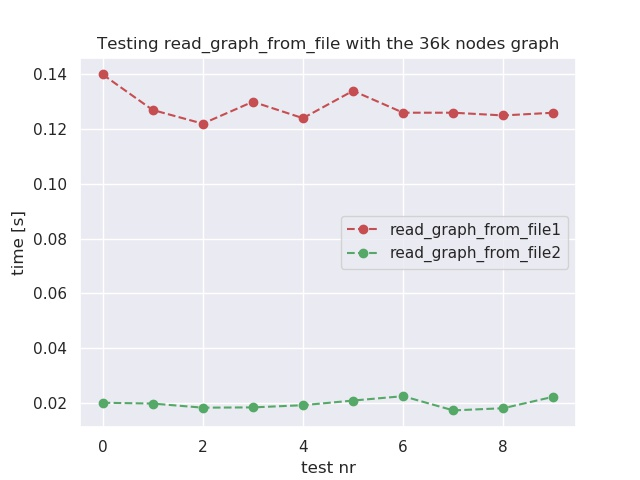
\includegraphics[width=15cm]{read_36k_graph.jpg}
%\caption{First.}
\label{fig:Test 1}}
\qquad
\caption{Tests the speed of our two files that reads the data. As we can see, the one where we implement the CRS-Format is more efficient  }
\end{figure}


\begin{figure}[H]
\centering
\parbox{15cm}{
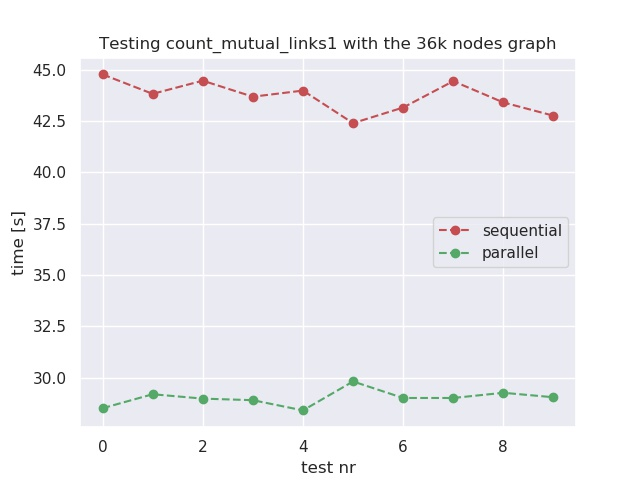
\includegraphics[width=15cm]{count_1_36k_graph.jpg}
%\caption{First.}
\label{fig:Test 1}}
\qquad
\caption{Here we counted mutual links using the data stored in the dense matrix. What we can see is that parallelizing gives a significant speedup. This speedup can be increased even more with more threads}
\end{figure}

\begin{figure}[H]
\centering
\parbox{15cm}{
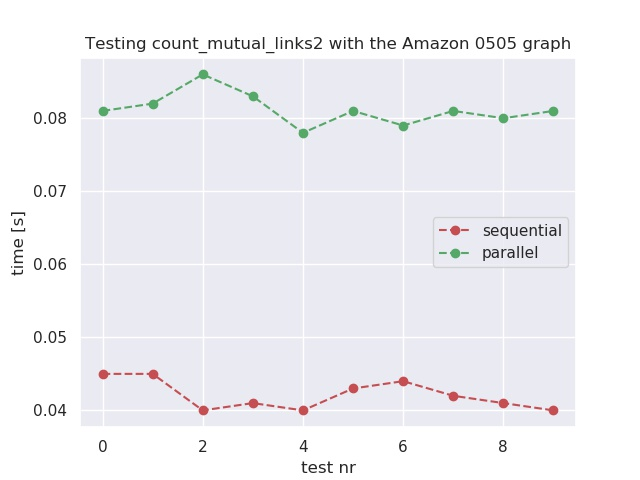
\includegraphics[width=15cm]{count_2_Amazon_graph.jpg}
%\caption{First.}
\label{fig:Test 1}}
\qquad
\caption{Here we counted mutual links using the data stored in the CRS-Format. This program was running so efficient that I had to use the largest data-set I could find (Amazon5050).}
\end{figure}

\section{Conclusion}

The first thing noticed was that the CRS-Format is way more efficient when it comes to computation. This can be seen by comparing Table 2 and Table 3.The dense matrix method did not work with large files like the \textit{web-NotreDame.txt} file, because of memory limitations, therefore, for big files, we had to use the CRS-Format method. \\
Besides that, parallelizing made a significant difference in computation speed when using the dense matrix implementation. The computation could have been improved even more if I would have had access to more threads. Moreover, parallelization did not decrease the time for computation when CRS-Format was used. This is likely because the computations were so fast that OpenMP made no difference.\\
In conclusion, the CRS-Format was shown to be superior in therms of computation speed compared to the dense matrix. But, in terms of parallelization, the files were too small for OpenMP to make a difference. Therefore, I cannot conclude that a speedup will be gained by parallelizing the CRS-Format function, but the possibility it will is likely.

\bibliographystyle{plain}
\bibliography{references}
\end{document}

